% Options for packages loaded elsewhere
\PassOptionsToPackage{unicode}{hyperref}
\PassOptionsToPackage{hyphens}{url}
\PassOptionsToPackage{dvipsnames,svgnames,x11names}{xcolor}
\documentclass[
  11pt,
]{article}
\usepackage{xcolor}
\usepackage[margin=2.2cm]{geometry}
\usepackage{amsmath,amssymb}
\setcounter{secnumdepth}{-\maxdimen} % remove section numbering
\usepackage{iftex}
\ifPDFTeX
  \usepackage[T1]{fontenc}
  \usepackage[utf8]{inputenc}
  \usepackage{textcomp} % provide euro and other symbols
\else % if luatex or xetex
  \usepackage{unicode-math} % this also loads fontspec
  \defaultfontfeatures{Scale=MatchLowercase}
  \defaultfontfeatures[\rmfamily]{Ligatures=TeX,Scale=1}
\fi
\usepackage{lmodern}
\ifPDFTeX\else
  % xetex/luatex font selection
\fi
% Use upquote if available, for straight quotes in verbatim environments
\IfFileExists{upquote.sty}{\usepackage{upquote}}{}
\IfFileExists{microtype.sty}{% use microtype if available
  \usepackage[]{microtype}
  \UseMicrotypeSet[protrusion]{basicmath} % disable protrusion for tt fonts
}{}
\makeatletter
\@ifundefined{KOMAClassName}{% if non-KOMA class
  \IfFileExists{parskip.sty}{%
    \usepackage{parskip}
  }{% else
    \setlength{\parindent}{0pt}
    \setlength{\parskip}{6pt plus 2pt minus 1pt}}
}{% if KOMA class
  \KOMAoptions{parskip=half}}
\makeatother
\usepackage{longtable,booktabs,array}
\usepackage{caption}
\captionsetup[table]{skip=6pt}
\newcounter{none} % for unnumbered tables
\usepackage{calc} % for calculating minipage widths
% Correct order of tables after \paragraph or \subparagraph
\usepackage{etoolbox}
\makeatletter
\patchcmd\longtable{\par}{\if@noskipsec\mbox{}\fi\par}{}{}
\makeatother
\usepackage{graphicx}
\makeatletter
\newsavebox\pandoc@box
\newcommand*\pandocbounded[1]{% scales image to fit in text height/width
  \sbox\pandoc@box{#1}%
  \Gscale@div\@tempa{\textheight}{\dimexpr\ht\pandoc@box+\dp\pandoc@box\relax}%
  \Gscale@div\@tempb{\linewidth}{\wd\pandoc@box}%
  \ifdim\@tempb\p@<\@tempa\p@\let\@tempa\@tempb\fi% select the smaller of both
  \ifdim\@tempa\p@<\p@\scalebox{\@tempa}{\usebox\pandoc@box}%
  \else\usebox{\pandoc@box}%
  \fi%
}
% Set default figure placement to htbp
\def\fps@figure{htbp}
\makeatother
\setlength{\emergencystretch}{3em} % prevent overfull lines
\providecommand{\tightlist}{%
  \setlength{\itemsep}{0pt}\setlength{\parskip}{0pt}}
\usepackage{fvextra}
\directlua{luaotfload.add_fallback("fb", {"STIX Two Text:mode=harf;", "STIX Two Math:mode=harf;", "Apple Symbols:mode=harf;", "Hiragino Sans:mode=harf;", "Menlo:mode=harf;", "Arial Unicode MS:mode=harf;"})}
\setmainfont{Latin Modern Roman}[RawFeature={fallback=fb}]
\setsansfont{Latin Modern Sans}[RawFeature={fallback=fb}]
\setmonofont{Latin Modern Mono}[RawFeature={fallback=fb}]
\usepackage{xurl}
\setlength{\emergencystretch}{3em}
\renewcommand{\arraystretch}{1.15}
\usepackage{bookmark}
\IfFileExists{xurl.sty}{\usepackage{xurl}}{} % add URL line breaks if available
\urlstyle{same}
% fallback for those not using the hyperref driver hyperxmp:
\makeatletter
\@ifundefined{xmpquote}{\newcommand{\xmpquote}[1]{#1}}{}
\makeatother
\hypersetup{
  pdftitle={md2pdf-latex: example document},
  colorlinks=true,
  linkcolor={blue!50!black},
  filecolor={Maroon},
  citecolor={Blue},
  urlcolor={blue!50!black},
  pdfcreator={LaTeX via pandoc}}

\title{md2pdf-latex: example document}
\author{}
\date{}

\begin{document}
\maketitle

This page is written in plain Markdown and typeset by LaTeX. Inline math
like \(e^{i\pi} + 1 = 0\) or
\(\mathrm{softmax}(x)_i = e^{x_i} / \sum_j e^{x_j}\) uses real TeX, and
so does display math:

\[\mathrm{Attention}(Q, K, V) = \mathrm{softmax}\!\left(\frac{QK^\top}{\sqrt{d_k}}\right) V\]

\section{Tables sized from their
content}\label{tables-sized-from-their-content}

A narrow table keeps its natural width:

{\def\LTcaptype{none} % do not increment counter
\begin{longtable}[]{@{}ll@{}}
\toprule\noalign{}
Symbol & Meaning \\
\midrule\noalign{}
\endhead
\bottomrule\noalign{}
\endlastfoot
\(d\) & model width \\
\(T\) & sequence length \\
\end{longtable}
}

A wide table shares the line between its columns, so long names never
overlap and text wraps only where needed:

\begingroup\small

{\def\LTcaptype{none} % do not increment counter
\begin{longtable}[]{@{}
  >{\raggedright\arraybackslash}p{(\linewidth - 10\tabcolsep) * \real{0.2951}}
  >{\raggedright\arraybackslash}p{(\linewidth - 10\tabcolsep) * \real{0.3315}}
  >{\raggedright\arraybackslash}p{(\linewidth - 10\tabcolsep) * \real{0.0937}}
  >{\raggedright\arraybackslash}p{(\linewidth - 10\tabcolsep) * \real{0.0585}}
  >{\raggedright\arraybackslash}p{(\linewidth - 10\tabcolsep) * \real{0.0585}}
  >{\raggedright\arraybackslash}p{(\linewidth - 10\tabcolsep) * \real{0.1252}}@{}}
\toprule\noalign{}
\begin{minipage}[b]{\linewidth}\raggedright
Experiment name
\end{minipage} & \begin{minipage}[b]{\linewidth}\raggedright
What changed
\end{minipage} & \begin{minipage}[b]{\linewidth}\raggedright
Learning rate
\end{minipage} & \begin{minipage}[b]{\linewidth}\raggedright
Batch
\end{minipage} & \begin{minipage}[b]{\linewidth}\raggedright
Steps
\end{minipage} & \begin{minipage}[b]{\linewidth}\raggedright
Result
\end{minipage} \\
\midrule\noalign{}
\endhead
\bottomrule\noalign{}
\endlastfoot
\texttt{baseline\_small\_model\_run} & nothing: the reference
configuration everyone else is compared to & 0.001 & 32 & 5,000 &
finished normally \\
\texttt{wider\_ffn\_variant\_run} & feed-forward layer made twice as
wide, everything else unchanged & 0.001 & 32 & 5,000 & finished
normally \\
\texttt{huge\_learning\_rate\_run} & learning rate raised far beyond the
stable range & 0.3 & 32 & 694 & diverged \\
\end{longtable}
}

\endgroup

\section{Code that wraps}\label{code-that-wraps}

\begin{Verbatim}[breaklines,breakanywhere,fontsize=\small,frame=leftline,framerule=0.6pt,rulecolor=\color{black!25},xleftmargin=4pt]
def a_function_with_a_rather_long_signature(first_argument, second_argument, third_argument, fourth_argument=None):
    return [first_argument, second_argument, third_argument, fourth_argument]  # long lines wrap instead of running off the page
\end{Verbatim}

\section{Colored blocks}\label{colored-blocks}

\begingroup\color[HTML]{2E8B57}

\textbf{Answer:} an HTML
\texttt{\textless{}div\ style="color:\#RRGGBB"\textgreater{}} around
Markdown becomes a colored block in the PDF, which is handy for telling
answers apart from questions.

\endgroup

\section{Figures with labels}\label{figures-with-labels}

\par\noindent\begin{minipage}{\linewidth}

\textbf{Learning curve:}

\begin{center}

\pandocbounded{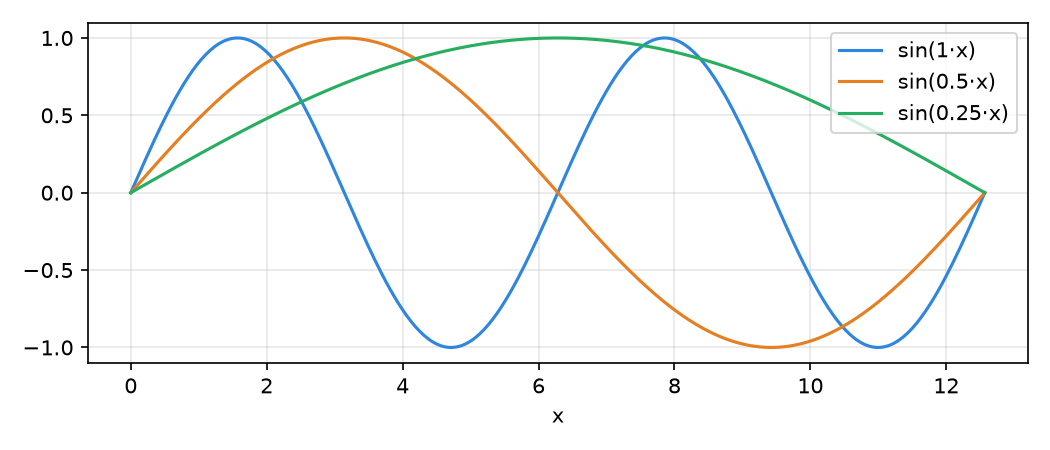
\includegraphics[keepaspectratio,alt={Three sine
waves}]{waves.png}}

\end{center}\end{minipage}\par\medskip

\emph{A label and its figure are kept together on one page, and the
figure is centered.}

\section{Unicode}\label{unicode}

Arrows and symbols → ≈ × ✓ ⚠, subscripts like ω\textsubscript{k},
accents (Ünïcödé), and other scripts (こんにちは) all render, thanks to
a chain of fallback fonts.

\end{document}
